\documentclass[tikz,border=0pt,11pt]{standalone}
\usepackage[T1]{fontenc}
\usepackage[utf8]{inputenc}
\usepackage{lmodern,amsmath,amssymb}
\usepackage[swedish]{babel}
\usetikzlibrary{arrows.meta,calc,positioning,decorations.pathmorphing,decorations.pathreplacing,patterns,shadings}
\definecolor{navy}{HTML}{102F40}
\definecolor{teal}{HTML}{147D78}
\definecolor{lightteal}{HTML}{E6F1ED}
\definecolor{gold}{HTML}{B88B3B}
\definecolor{palegold}{HTML}{F7EEDB}
\definecolor{rust}{HTML}{B6533B}
\definecolor{palerust}{HTML}{FAEAE4}
\definecolor{paper}{HTML}{F7F5EE}
\definecolor{muted}{HTML}{5B6D72}
\definecolor{line}{HTML}{D6DED8}
\renewcommand{\familydefault}{\sfdefault}
\newcommand{\atom}[5]{\shade[ball color=#3!70] (#1,#2) circle (#5);\node[text=white,font=\bfseries\small] at (#1,#2){#4};}
\newcommand{\water}[3]{\begin{scope}[shift={(#1,#2)},scale=#3]\draw[navy!45,line width=2pt] (-.3,.22)--(0,0)--(.3,.22);\atom{0}{0}{rust}{O}{.22}\atom{-.3}{.22}{teal}{H}{.15}\atom{.3}{.22}{teal}{H}{.15}\end{scope}}
\newcommand{\panel}[4]{\filldraw[fill=white,draw=line,rounded corners=5pt] (#1,#2) rectangle ++(#3,#4);}
\newcommand{\note}[4]{\node[txt,text width=#3cm] at (#1,#2){#4};}
\tikzset{txt/.style={anchor=north west,align=left,text=navy,font=\small},
 head/.style={anchor=west,text=navy,font=\bfseries\large},
 label/.style={align=center,text=navy,font=\small},
 smalllabel/.style={align=center,text=muted,font=\footnotesize},
 arrow/.style={-{Latex[length=2.5mm,width=1.8mm]},line width=1.2pt,draw=teal},
 goldarrow/.style={-{Latex[length=2.5mm]},line width=1.2pt,draw=gold},
 rustarrow/.style={-{Latex[length=2.5mm]},line width=1.2pt,draw=rust},
 dashedarrow/.style={arrow,dashed},
 badge/.style={fill=lightteal,rounded corners=3pt,text=teal,font=\bfseries\small,inner sep=5pt}}
\begin{document}
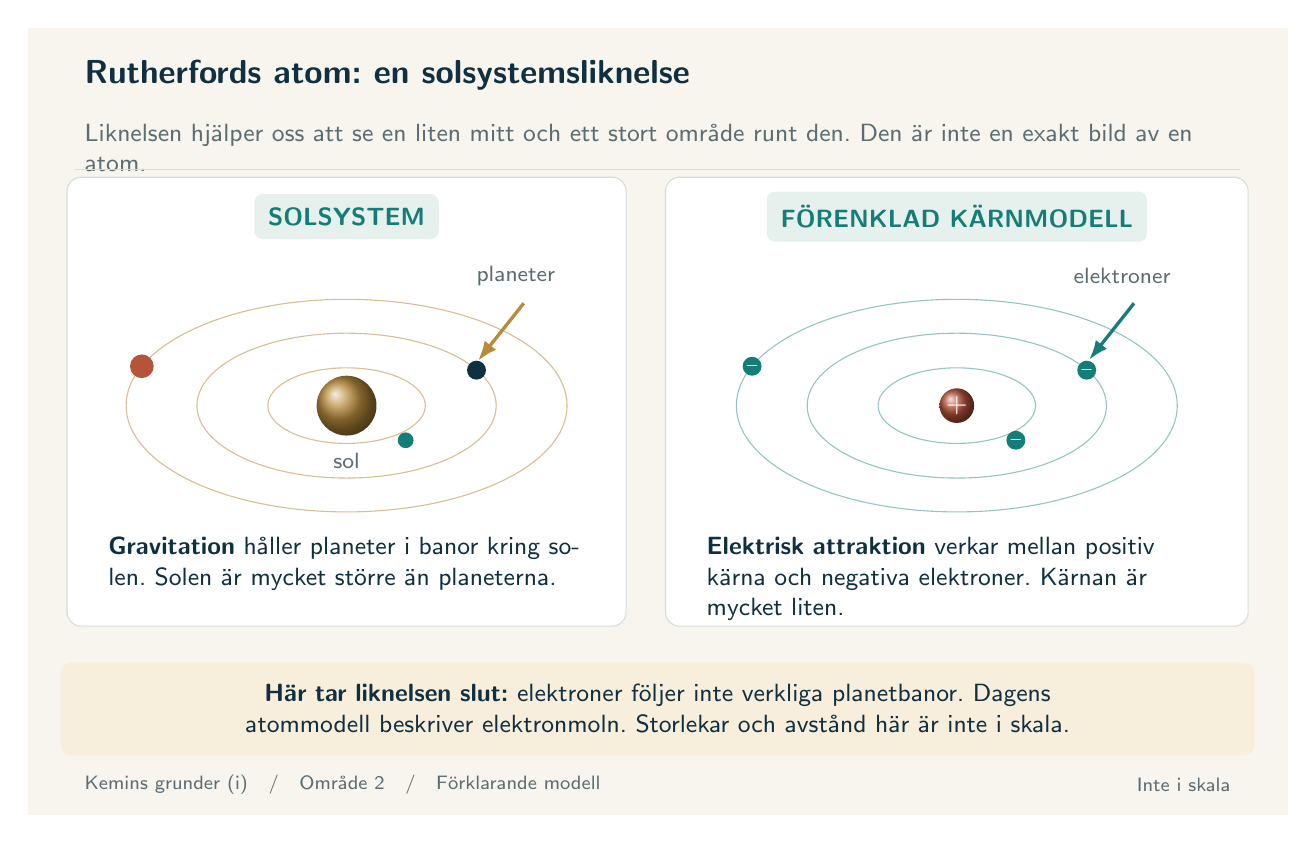
\begin{tikzpicture}[x=1cm,y=1cm]
\path[use as bounding box] (0,0) rectangle (16,10);
\fill[paper] (0,0) rectangle (16,10);
\node[head] at (.6,9.4){Rutherfords atom: en solsystemsliknelse};
\note{.6}{8.9}{14.8}{\textcolor{muted}{Liknelsen hjälper oss att se en liten mitt och ett stort område runt den. Den är inte en exakt bild av en atom.}}
\draw[line] (.6,8.2)--(15.4,8.2);

\panel{.5}{2.4}{7.1}{5.7}\panel{8.1}{2.4}{7.4}{5.7}
\node[badge] at (4.05,7.6){SOLSYSTEM};\node[badge] at (11.8,7.6){FÖRENKLAD KÄRNMODELL};
\foreach \rx/\ry in {1/.48,1.9/.92,2.8/1.35}{\draw[gold!55] (4.05,5.2) ellipse[x radius=\rx cm,y radius=\ry cm];\draw[teal!45] (11.8,5.2) ellipse[x radius=\rx cm,y radius=\ry cm];}
\shade[ball color=gold] (4.05,5.2) circle(.38);\node[smalllabel] at (4.05,4.5){sol};
\fill[navy] (5.7,5.65) circle(.12);\fill[rust] (1.45,5.7) circle(.15);\fill[teal] (4.8,4.76) circle(.1);
\shade[ball color=rust] (11.8,5.2) circle(.22);\node[text=white,font=\bfseries] at (11.8,5.2){$+$};
\foreach \x/\y in {13.45/5.65,9.2/5.7,12.55/4.76}{\fill[teal] (\x,\y) circle(.12);\node[text=white,font=\tiny] at (\x,\y){$-$};}
\draw[goldarrow] (6.3,6.5)--(5.72,5.77);\node[smalllabel,text width=2cm] at (6.2,6.85){planeter};
\draw[arrow] (14.05,6.5)--(13.48,5.78);\node[smalllabel,text width=2.3cm] at (13.9,6.85){elektroner};
\note{.9}{3.65}{6.2}{\textbf{Gravitation} håller planeter i banor kring solen. Solen är mycket större än planeterna.}
\note{8.5}{3.65}{6.3}{\textbf{Elektrisk attraktion} verkar mellan positiv kärna och negativa elektroner. Kärnan är mycket liten.}
\node[label,text width=14.6cm,fill=palegold,rounded corners=4pt,inner sep=8pt] at (8,1.35){\textbf{Här tar liknelsen slut:} elektroner följer inte verkliga planetbanor. Dagens atommodell beskriver elektronmoln. Storlekar och avstånd här är inte i skala.};\node[anchor=west,text=muted,font=\scriptsize] at (.6,.38){Kemins grunder (i)\quad /\quad Område 2\quad /\quad Förklarande modell};
\node[anchor=east,text=muted,font=\scriptsize] at (15.4,.38){Inte i skala};
\end{tikzpicture}\end{document}
